\documentclass[12pt,twoside]{rif}

\pagestyle{myheadings}
\usepackage[
left=2.54cm,
right=2.54cm,
top=2.54cm,
bottom=2.54cm]
{geometry}
\usepackage{hyperref}
\usepackage{natbib}
\usepackage{subfigure}
\hypersetup{
	urlcolor=blue, 
	colorlinks=true, 
	citecolor=blue
}

\usepackage{lipsum}

\title{\textbf{Dilatación del tiempo gravitacional}}

\author[1]{{\small Carlos Andrés García Suarez}} 
\author[1]{{\small David Brandon Zevallos Garay}}
\author[1]{{\small Luis Fernando Ubillus Benites}}
%\author[3]{Autor3}
\affil[1]{{ \small Facultad de Ciencias Naturales y Matemática, Universidad
		Nacional Federico Villarreal. El Agustino 15003. Lima-Perú.}}
%\affil[2,3]{Afiliacion2}
%\date{\normalsize Recibido: xxxx Aceptado: xxxx Publicado: xxxx\\
%Todos los derechos reservados-SEF \copyright{} 2012}
\date{}

\begin{document}
	\maketitle
	
	\begin{res}
		\begin{center}
			\textbf{Resumen} \\
		\end{center}
		\lipsum[2]
		
		\par
		\smallskip
		\clav{sdjssasdfsdf, asdfsdf, asdfsdafsd}
	\end{res}
	\begin{center}
		\title{\textbf{Time gravitational dilation}}
	\end{center}
	
	\begin{abst}
		\begin{center}
			\textbf{Abstract} \\
		\end{center}
		\lipsum[2]
		
		\par 
		\smallskip
		\key{sdjssasdfsdf, asdfsdf, asdfsdafsd}
	\end{abst}

	
	
	\newpage
	
	\tableofcontents
	
	\section{ Introducción} 
	\subsection{Transformadas de Galileo}
	Una de los primeros indicios a nivel historico de relatividad fue propuesto 
	por Galileo, el principio de relatividad de Galileo establece que:
	Dos sistemas de referencia en movimiento relativo de traslación rectilínea 
	uniforme son equivalentes desde el punto de vista mecánico; es decir, los experimentos 
	mecánicos se desarrollan de igual manera en ambos, y las leyes de la mecánica son las mismas.

    Suponga que se presenta algún fenómeno físico, que llamará evento, el cual es observado por alguien en reposo en un marco inercial de referencia. Al decir que un observador está “en un marco”, significa que está en reposo respecto al origen de ese marco. La
    ubicación y tiempo del evento pueden ser especificados por las cuatro coordenadas (x, y,
    z, t). Lo deseable es poder transformar las coordenadas de un observador en un marco
    inercial a las de otro en un marco que se mueve con velocidad relativa uniforme en comparación con el primer marco.

	\begin{figure}[h!]
		\centering
		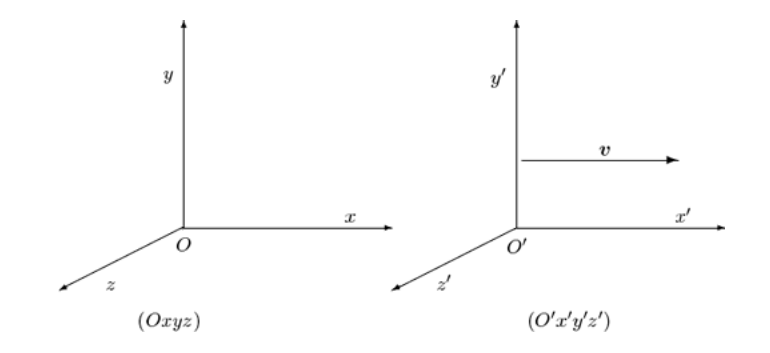
\includegraphics[width=0.7\textwidth]{img/Galileo.PNG}
		\caption{Sistemas de referencia en movimiento relativo rectilíneo
		y uniforme, con velocidad $v$ en dirección $O_{x}$ }
		\label{fig:01}
		\end{figure}

		Como muestra la geometría de la figura \ref*{fig:01}, las relaciones entre estas coordenadas se escriben 
		como:
		\begin{align*}
			x'&=x-vt\\
			y'&=y\\
			z'&=z\\
			t'&=t\\
		\end{align*}

		Éstas son las ecuaciones de transformación galileanas del espacio–tiempo. Observe que
		el tiempo se supone el mismo en ambos marcos inerciales; es decir, dentro de la estructura de la mecánica clásica, todos los relojes funcionan al mismo ritmo, cualquiera que
		sea su velocidad, de modo que el tiempo en el que se presenta un evento para un observador en S es el mismo tiempo para el mismo evento en S9. En consecuencia, el intervalo
		de tiempo entre dos eventos sucesivos debe ser el mismo para ambos observadores.
\newpage
	\subsection{Transformadas de Lorentz}
	\subsection{Diagrama Minkowski}
	
	
	
	\section{Marco Teórico}

	
		
	\section{Conclusiones}
	
	\nocite{*}
	\bibliographystyle{apa}
	\bibliography{biblio}
	

\end{document}